\documentclass[a4paper, 12pt]{article}

\usepackage[czech]{babel}
\usepackage[utf8]{inputenc}

%show the geometry of pages on top of every page
% \usepackage{showframe}

%for bib overfull hbox
\usepackage{xurl}

%math
\usepackage{amsmath}

%biblatex bibliography
\usepackage{csquotes}
\usepackage[backend = biber, sorting = none, giveninits, style = authoryear, defernumbers = true, uniquename = init]{biblatex}
%name order
\DeclareNameAlias{default}{family-given}
\DeclareNameAlias{sortname}{family-given}
%add comma between author and year in citations
\renewcommand*{\nameyeardelim}{\addcomma\space}
%change url: to dostupné z
\DeclareFieldFormat{url}{Dostupné z\space\url{#1}}
%create \citejournal
\DeclareCiteCommand{\citejournal}
  {\usebibmacro{prenote}}
  {\usebibmacro{citeindex}%
    \usebibmacro{journal}}
  {\multicitedelim}
  {\usebibmacro{postnote}}
%get rid of In: before journal title
\renewbibmacro{in:}{}
%change and to ampersand in author citation
\AtBeginBibliography{%
  \renewcommand*{\finalnamedelim}{%
    \ifnumgreater{\value{liststop}}{2}{\finalandcomma}{}%
    \addcomma\addspace\&\space}%
}

%
%add the bib file
\addbibresource{citations.bib}
%for biblatex to work with inputenc
\usepackage[T1]{fontenc}
\usepackage{textcomp}

%bold math
\usepackage{bm}

%graphics
\usepackage{graphicx}

%layout and spacing
\usepackage[lmargin=3.5cm, rmargin=2.5cm, tmargin=2.5cm, bmargin=2.5cm]{geometry}

%lineheight 1.5
\usepackage{setspace}
\onehalfspacing

%paragraph spacing
\usepackage[skip=6pt]{parskip}

%tikz for graphs and math figures
\usepackage{tikz}
\usepackage{etoolbox} % ifthen
\usepackage[outline]{contour} % glow around text
\usetikzlibrary{calc} % for adding up coordinates
\usetikzlibrary{decorations.markings,decorations.pathmorphing}
\usetikzlibrary{angles,quotes} % for pic (angle labels)
\usetikzlibrary{arrows.meta} % for arrow size
\usepackage{xfp} % higher precision (16 digits?)
\usetikzlibrary{angles, quotes}
\usetikzlibrary{shapes.geometric}

%styles for spacetime diagrams
\newcommand{\calI}{\mathscr{I}} %\mathcal
\tikzset{>=latex} % for LaTeX arrow head
%\colorlet{mylightbrown}{brown!70!red!70!black!12}
\tikzstyle{world line}=[draw = gray,line width=0.3]
\tikzstyle{world line t}=[draw = gray,line width=0.3]
\tikzstyle{world line'}=[draw = black,line width=0.3]
\tikzstyle{mysmallarr}=[-{Latex[length=3,width=2]},thin]
\tikzstyle{mydashed}=[dash pattern=on 3 off 3]
\tikzstyle{rod}=[mydarkbrown,draw=mydarkbrown,double=mybrown,double distance=2pt,
                 line width=0.2,line cap=round,shorten >=1pt,shorten <=1pt]
\tikzstyle{vector}=[->,line width=1,line cap=round]
\tikzstyle{vector'}=[vector,shorten >=1.2]
\tikzstyle{particle}=[mygreen,line width=0.9]
\tikzstyle{photon}=[-{Latex[length=5,width=4]},black,line width=0.8,decorate,
                    decoration={snake,amplitude=1.0,segment length=5,post length=5}]

\def\tick#1#2{\draw[thick] (#1) ++ (#2:0.06) --++ (#2-180:0.12)}
\def\tickp#1#2{\draw[thick,mydarkred] (#1) ++ (#2:0.06) --++ (#2-180:0.12)}
\def\Nsamples{100}

%add date (year command for title page)
\usepackage{datetime}
\newdateformat{yeardate}{\THEYEAR}

%for adding unnumbered sections to TOC
\usepackage{hyperref}

%new section new page
\AddToHook{cmd/section/before}{\clearpage}


\title{Superdeterminismus}
\author{Kryštof Pšenička}

%title page
\makeatletter
\def\@maketitle{%
  \newpage
  \null
  \vskip 2em%
  \begin{center}%
  \begin{figure}[ht]
    \centering
    
\includegraphics[width=230pt]{images/gymck-logo.png}
\end{figure}
    {\huge \textbf{SEMINÁRNÍ PRÁCE} \par}%
    \vskip 2.5em%
    {\Large
      \lineskip .5em%
      \begin{tabular}[t]{c}%
        \@author
      \end{tabular}\par}%
    \vskip 1em%
    {\Large \textbf{\@title} \par}%
    \vskip 6em%
    {\large Vedoucí seminární práce: Mgr. Ivana Špilínková \par}%
    \vskip 5em%
    {\yeardate\today}%
  \end{center}%
  \par
  \vskip 1.5em}
\makeatother

%acknowledgements
\def\acknowledgements{%
  \newpage
  \null
  \vskip 2em%
    {\large \textbf{Poděkování} \par}
    {Chtěl bych poděkovat své vedoucí seminární práce Mgr. Ivaně Špilínkové za odborné vedení, za pomoc, za gramatickou kontrolu a rady při zpracování této práce.}
  }%

%sworn declaration
\def\makesworndec{%
  \newpage
  \null
  \vskip 40em%
    {Prohlašuji, že jsem tuto seminární práci vypracoval samostatně a výhradně\par s použitím citovaných pramenů, literatury a dalších odborných zdrojů. \par}%
    \vskip 5em%
    {V ..................... dne .....................}%
  \par
  \vskip 1.5em}



\begin{document}

\maketitle
\thispagestyle{empty}

\makesworndec
\thispagestyle{empty}

\acknowledgements
\thispagestyle{empty}

\tableofcontents
\thispagestyle{empty}

\clearpage

\pagenumbering{arabic} 
\section{Úvod}
(Zpracováno podle knihy \cite{quantum})

Na konci 19. století se vědci domnívali, že s výjimkou několika detailů jejich teorie dokázaly odpovědět na všechny otázky fyziky. Podle nich už na obzoru nebyly žádné velké objevy. Maxwellovy rovnice elektromagnetismu a Newtonovy pohybové zákony kreslily deterministický vesmír, v němž má každá částice určitou pozici a momentum v daném okamžiku. Síly které působí na částici určují, jak se její pozice a rychlost mění v čase.

Ale už v roce 1900, při řešení problému absolutně černého tělesa, objevil Max Planck kvanta - nedělitelné balíky světla, jejichž velikost (energie) závisí na frekvenci daného světla. I když si v té době Max Planck i většina ostatních fyziků myslela, že to je pouze matematický trik, který nemá žádné implikace ve fyzickém světě, byl to první krok vedoucí ke kvantové revoluci.

Albert Einstein věřil ve fyzickou existenci Planckových kvant a ve vlnově-korpusku\-lární dualitu světla, podle níž je světlo částicí a vlnou zároveň a chová se jako jedno nebo druhé podle způsobu našeho pozorování. Ve svém Annus mirabilis\footnote[1]{Zázračný rok, ve kterém Einstein vydal 4 revoluční vědecké články.} (1905) kvantově vysvětlil fotoefekt: když elektron získá dostatek energie absorbcí kvanta světla, je uvolněn z obalu atomu a následně může být vyzařován.

Francouzský aristokrat Luis de Broglie vzal tento závěr z Planckovy práce ještě dál a teoretizoval o vlnově-korpuskulární dualitě všech částic, nejen světelných, ale také částic hmotných.

Kvantový model atomu se postupně vyvíjel od modelu Nielse Bohra s jedním kvantovým číslem, vyjadřujícím velikost oběžné dráhy elektronu. Arnold Sommerfeld postupně k tomuto modelu přidal 3 další kvantová čísla: jedno vyjadřující tvar eliptické oběžné dráhy elektronu, druhé (magnetické) vyjadřující orientaci oběžné dráhy v prostoru a poslední vyjadřující spin, což je vnitřní moment hybnosti částice.

V této době bylo zřejmé, že je potřeba vytvořit teorii, která by popisovala fenomény kvantového světa: kvantovou mechaniku.

Roku 1925 Werner Heisenberg přišel na Maticovou kvantovou mechaniku. Maticová, protože ve výpočtech využívá matic a vektorů. Matice jsou tabulky čísel (viz Obrázek \ref{fig:1}), které v této teorii mohou vyjadřovat veličiny jako polohu a hybnost částice. Vektory jsou veličiny, které mají kromě velikosti i směr a dají se vyjádřit maticemi. V Maticové mechanice se používají k vyjádření stavu systému. Vzhledem k používaným matematickým prostředkům je tato teorie nesmírně nepraktická k výpočtu vývoje jakéhokoli systému, jelikož rozměry matic se zvyšují exponenciálně s rostoucím počtem částic v systému.

\begin{figure}[ht]
    \centering
    $\begin{pmatrix}
    1 & 0 & 1 \\
    0 & 1 & 0 \\
    1 & 0 & 1
    \end{pmatrix}
    $
    \caption{\label{fig:1}Matice o 3 řádcích a 3 sloupcích.}
\end{figure}

Pouze tři měsíce po vydání Heisenbergova článku o Maticové mechanice zkonstruoval rakouský fyzik Erwin Schrödinger svou proslulou vlnovou rovnici (Rovnice (\ref{eq:1})), která popisuje vývoj vlnové funkce a stala se základem Schrödingerovy vlnové mechaniky. Vlnová mechanika se rychle stala oblíbenější než Maticová, jelikož výpočty s vlnovou rovnicí jsou daleko jednodušší.

\begin{equation}
    \bm{i\hbar \frac{\partial \Psi}{\partial t} = -\frac{\hbar^2}{2m}
    \frac{\partial^2 \Psi}{\partial x^2} + V \Psi}
    \label{eq:1}
\end{equation}

O rok později Schrödinger dokázal matematickou ekvivalenci Maticové a Vlnové mechaniky. Jsou to dvě formy téže teorie - Kvantové mechaniky.

Ve stejném roce Max Born předložil pravděpodobnostní interpretaci vlnové funkce, ve které druhá mocnina vlnové funkce vyjadřuje pravděpodobnostní distribuční funkci výsledku. Pro ilustraci vezměte v úvahu obrázek \ref{fig:2}. $\bm{\Psi}$ je vlnová funkce, která vyjadřuje stav systému, např. pozici elektronu. \textbf{P} je pravděpodobnostní distribuční funkce. Tato funkce vyjadřuje pravděpodobnost pro každý možný výsledek měření (každá možná pozice elektronu). $\bm{P(x_0,x_1)}$ je pravděpodobnost, že výsledek měření bude mezi $x_0$ a $x_1$. V našem případě je to pravděpodobnost, že elektron bude mít pozici mezi $x_0$ a $x_1$ a počítá se integrací pravděpodobnost\-ní funkce mezi hodnotami $x_0$ a $x_1$. Integrací $(\int_{x_0}^{x_1}|\Psi|^2\,dx)$ získáme obsah pod křivkou v daném rozsahu, který odpovídá hledané pravděpodobnosti. 


\clearpage

\begin{figure}[ht]
\centering
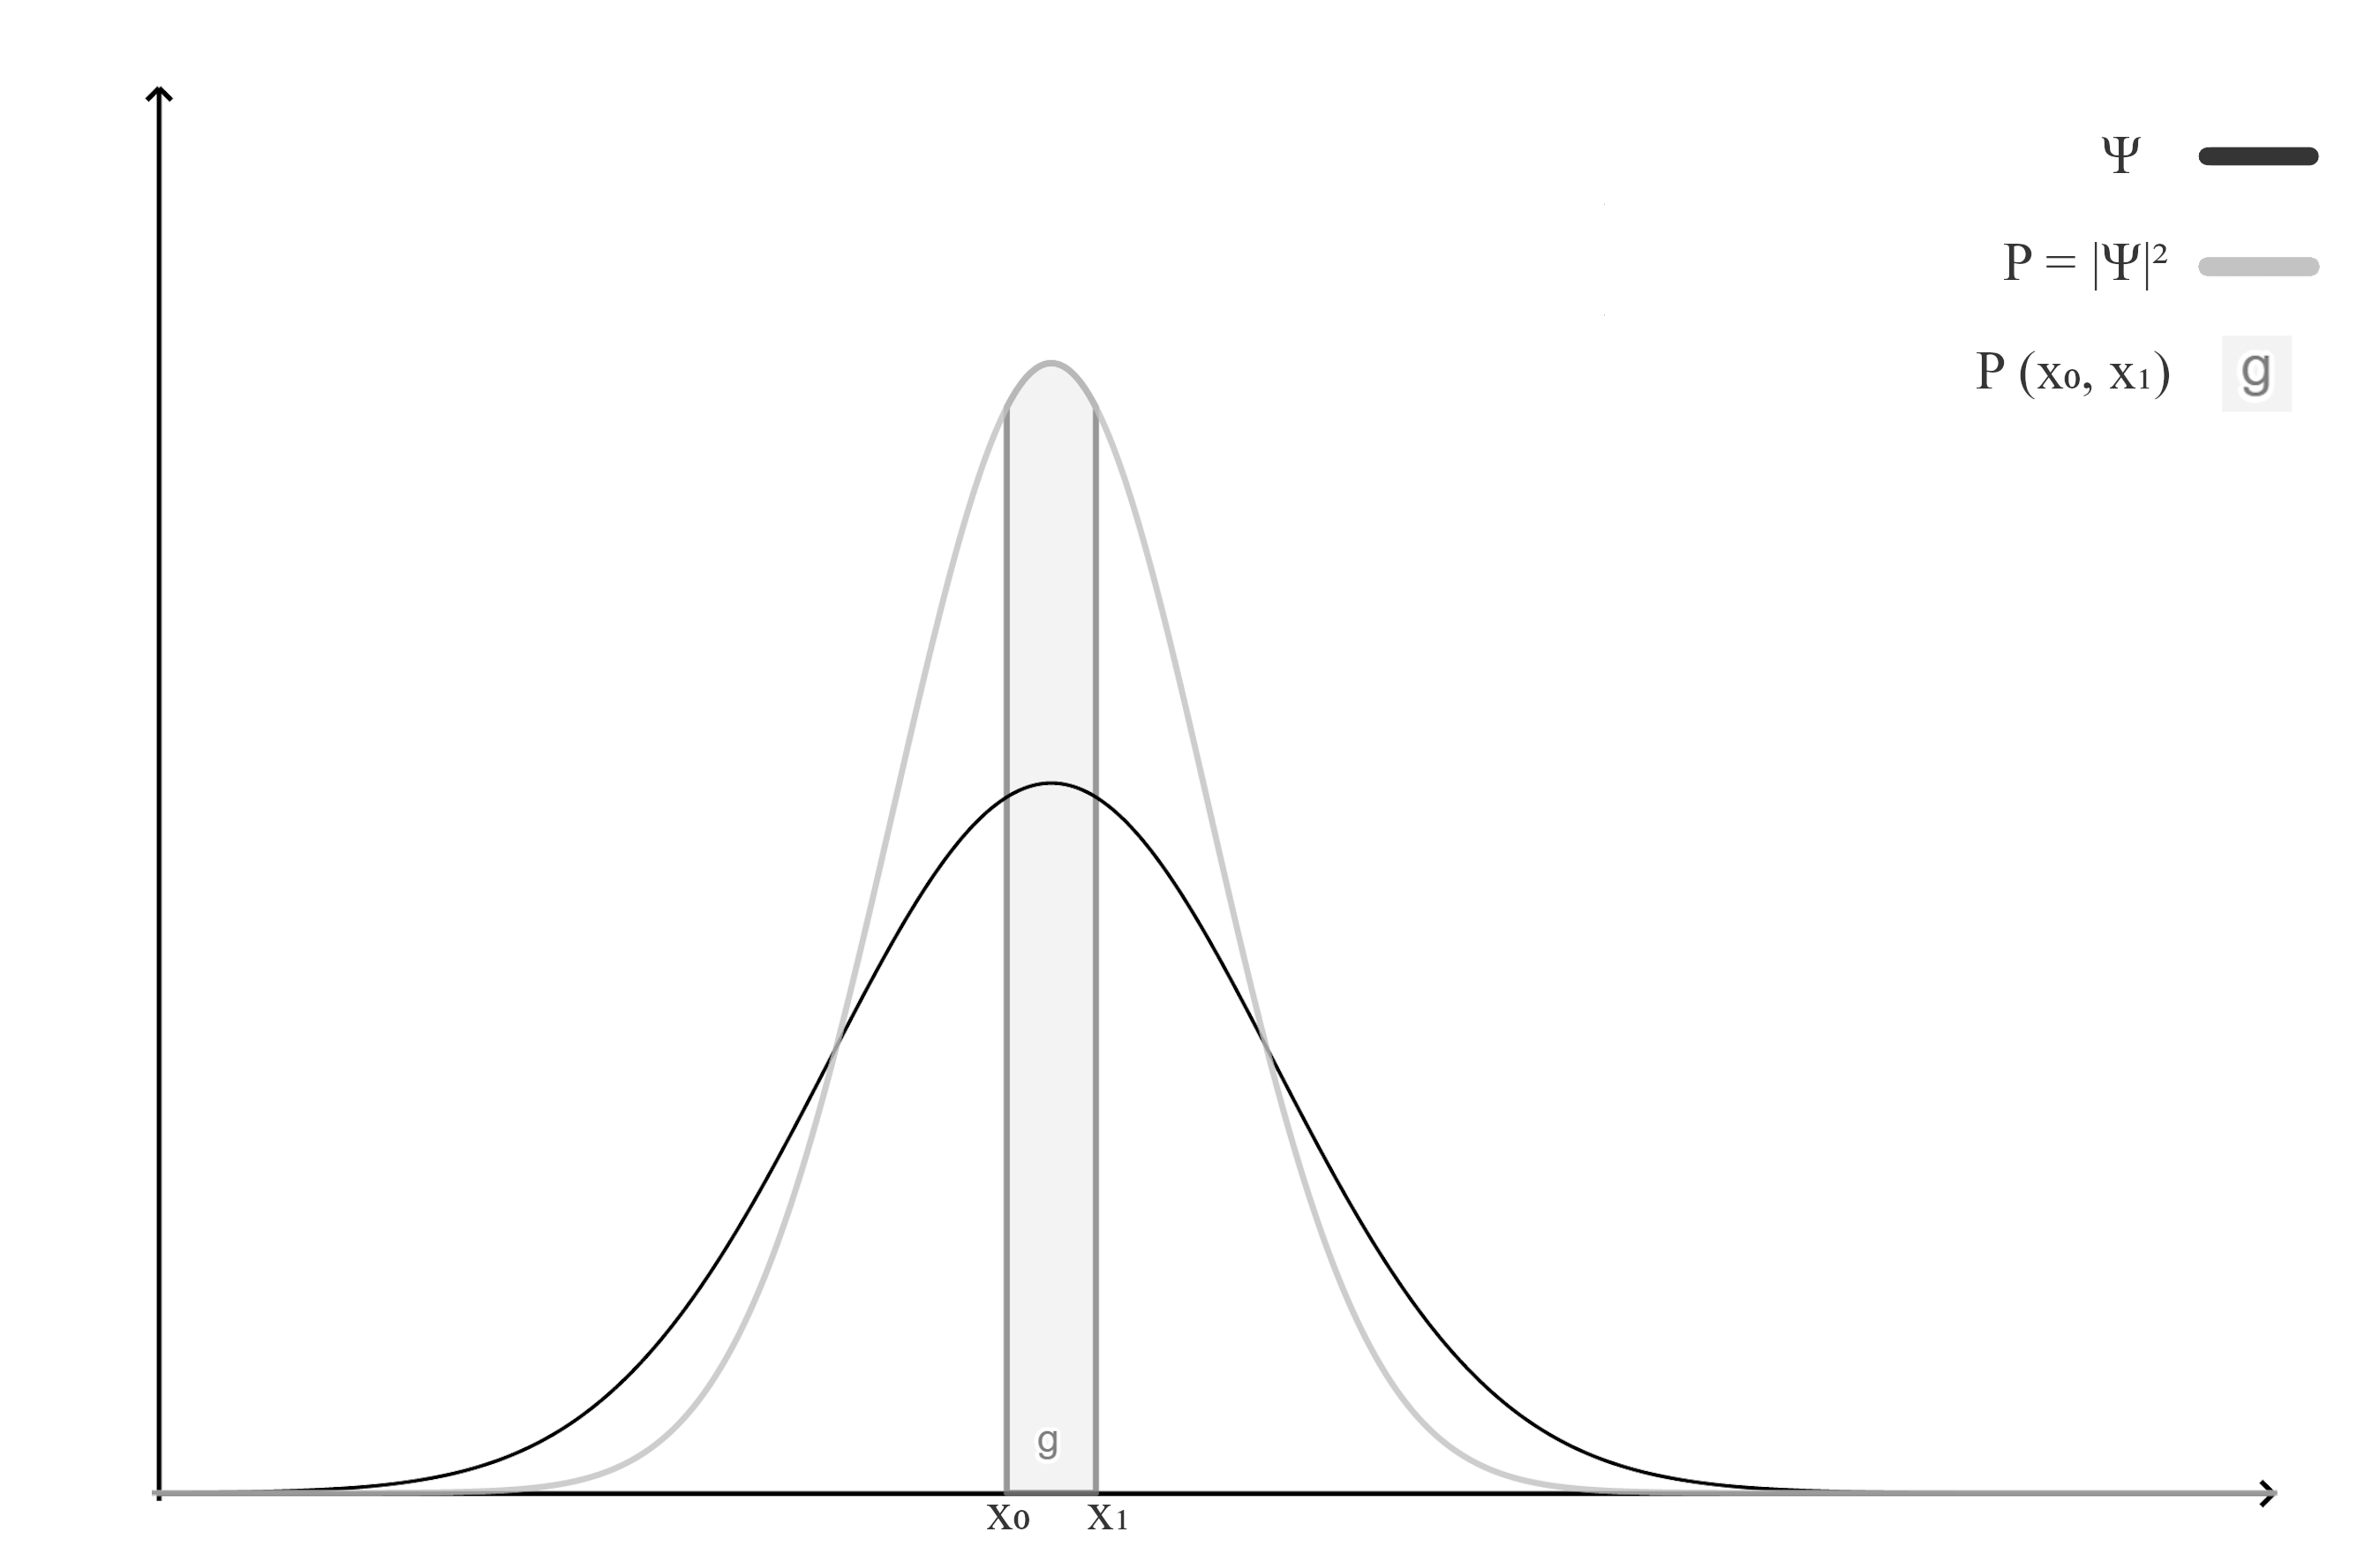
\includegraphics[width=300pt]{images/probability-function.png}
\caption{\label{fig:2}Vlnová funkce, pravděpodobnostní funkce a pravděpodobnost určitého výsledku.}
\end{figure}



Tato pravděpodobnostní interpretace se stala důležitou součástí dnešní Kvantové mechaniky, za kterou je považována Kodaňská interpretace, kterou společně vyhotovili Bohr, Pauli a Heisenberg v Bohrově institutu v Kodani.

Kvantová mechanika změnila obraz vesmíru z deterministického a předurčeného na indeterministický a pravděpodobnostní. V kvantovém pravděpodobnostním vesmíru můžeme určit pouze pravděpodobnost daného výsledku. Jediný způsob, jak Clerk Maxwell a Ludwig Boltzmann mohli popsat vlastnosti plynu skládajícího se z nesčetného množství částic bylo, použitím pravděpodob\-nosti a museli se spokojit se statistickým popisem. Tento nucený ústup ke statistické analýze byl způsoben neuskutečnitelností sledování pozice a rychlosti tolika částic. Pravděpodob\-nost byla důsledkem lidské nevědomosti. Naopak podle Kvantové mechaniky toto pravděpodobnost\-ní vyjádření kvantového světa není způsobeno lidskou nevědomostí, ale je fundamentální vlastností kvantového vesmíru.

Přes jeho účast v začátcích kvantové revoluce se Albert Einstein stal jejím největším kritikem. Uvědomoval si její užitečnost v atomových měřítcích, ale myslel si, že \uv{Bůh ne{hraje v }kostky.} Byl přesvědčený, že kvantová mechanika není konečnou teoríí, že za ní musí být fundamentálnější deterministická teorie. Takovým teoriím se říká teorie se \uv{skrytými} parametry. Podle těchto teorií dokážeme určit jen pravděpodobnost výsledků, jelikož neznáme všechny parametry. Kdybychom znali tyto \uv{skryté} parametry, dokázali bychom určit přesný výsledek měření.

V roce 1962 našel John Stewart Bell způsob, jak matematicky posoudit možnost teorie se skrytými parametry, která by replikovala výsledky kvantové mechaniky. Dnes se jí říká Bellova nerovnost. Tato nerovnost byla experimentálně porušena. Podle všeobecného mínění znamená porušení této nerovnosti nemožnost teorie se skrytými parametry. Toto porušení ale pouze znamená, že neexistuje teorie se skrytými parametry, která splňuje princip lokálního realismu a podmínku Statistické Nezávislosti.

V této práci se budu věnovat teorii se skrytými parametry, která nesplňuje podmínku Statistické Nezávislosti. Takovou teorii nazval Bell Superdeterminismus. Statistická Nezávislost (viz Rovnice (\ref{eq:2})) znamená, že pravděpodobnostní distribuce skrytých parametrů ($\bm{P(\lambda)}$) se nezmění, když vezmeme v potaz nastavení detektorů, \textbf{(a,b)}. Této podmínce se často říká podmín\-ka svobodné vůle, nebo svobodné volby. 

Cílem této práce je přehodnocení argumentů proti Superdeterminismu. Pokusím se vysvětlit, v rozporu s všeobecným míněním, že Superdeterminismus je cestou, která by mohla vyřešit mnoho problémů se současnými teoriemi a kterou bychom neměli ignorovat; je to cesta kterou jsme se nevydali.

\begin{equation}
    \bm{P(\lambda|\bm{a},\bm{b}) = P(\lambda)} 
    \label{eq:2}
\end{equation}



\input{partials/Problemy\_kvant\_mech.tex}
\input{partials/Bellova\_nerovnost.tex}
\section{Superdeterminismus}
\subsection{Definující vlastnosti}
(Zpracováno podle článku \cite{supdet:rethink})

Superdeterministické teorie jsou Psi-epistemické, deterministické a lokální teorie skrytých proměnných, které porušují Statistickou Nezávislost a nemusí být nutně realistické.

\subsubsection{Psi-epistemická}
Podle Psi-epistemické teorie vlnová funkce Schrödingerovy rovnice (Psi, $|\psi\rangle$) neodpovídá přímo vlastnosti nějakého systému v reálném světě. Kodaňská interpretace Kvantové mechaniky je Psi-epistemická, protože považuje vlnovou funkci pouze za reprezentaci znalostí o stavu systému.

Opakem je Psi-ontická teorie, která bere vlnovou funkci jako fundamentální část reálného světa.

Superdeterministické teorie jsou Psi-epistemické v tom smyslu, že vlnová funkce je průměrná pravděpodobnostní reprezentace přesných veličin systému, popsaných hlubší teorií.

Vlnová funkce odvozená ze superdeterministické teorie by se měla řídit dosud ověřenými evolučními zákony kvantové mechaniky. Smysl hledání takové teorie je tedy vytváření předpovědí nad rámec kvantové mechaniky.

\subsubsection{Deterministická}
Roku 1814 formuloval matematik Pierre-Simon de Laplace myšlenku deterministického vesmíru pomocí Laplaceova démona \parencite{laplace:demon}. Podle determinismu by bytost (démon) znající pozici a momentum každé částice ve vesmíru a mající dostatečnou výpočetní sílu mohla pomocí základních zákonů přírody vypočítat minulost i budoucnost každé částice. Vše je předurčené, evoluce každé částice je dána přírodními zákony.

Determinismem myslíme, že evoluční zákon teorie jednoznačně mapuje stavy systému v čase \textbf{\emph{t}} na stavy v čase \textbf{\emph{t'}} pro libovolné \textbf{\emph{t}} a \textbf{\emph{t'}}.

Jelikož Kvantová mechanika není deterministická, musí deterministická teorie reprodukující Kvantovou mechaniku obsahovat skryté proměnné. Skryté proměnné, nadále kolektivně označované $\bm{\lambda}$, obsahují všechny informace potřebné k určení výsledku měření kromě \uv{neskrytých} proměnných, které jsou obsaženy v přípravě stavu systému.

Je důležité poznamenat, že tyto skryté proměnné nemusí být vlastní pro měřený systém, ani v něm lokalizované. Představme si chlapce jménem Nikolaj, který má na mysli dvě otázky: \uv{Jaká je moje hmotnost?} a \uv{Zvládnu úspěšně udělat maturitní zkoušky?} V deterministickém vesmíru se odpovědi na obě otázky nacházejí v současném stavu vesmíru, ale jejich dostupnost je velmi odlišná. Informace o hmotnosti Nikolaje se vyskytuje lokálně v něm samotném, zatímco informace o jeho úspěšnosti při maturitní zkoušce je rozložena po většině prostoru současné chvíle.

\subsubsection{Lokální}
(Zpracováno podle článku \cite{CoA})

Lokalitou v Superdeterminismu exkluzivně myslíme Kontinuitu Působení (dále jen KoP). Zvažme oddělené časoprostorové oblasti $\bm{1}$ a $\bm{2}$ (viz Obrázek \ref{fig:7}), přičemž $\bm{1}$ je obklopena \uv{zastiňovací} oblastí $\bm{S}$. $\bm{S}$ není pouze prostorovou oblastí, zahrnuje budoucnost i minulost oblasti $\bm{1}$ a zároveň i její prostorový rozsah (v dimenzích $\bm{x,y,z}$).

\begin{figure}[ht]

    \centering

    \begin{tikzpicture}[scale=0.85]
        % S
        \draw (2, 4) circle (1.3);
        \draw (2, 4) circle (1);

        \draw[<-] (3.15, 4) -- (4, 3) node[below] (S) {$S$};
        
        %1
        \draw (2, 4) node  (1) {$1$};
        \draw (2, 4) circle (0.5);
        
        %2
        \draw (5.5, 3) node  (2) {$2$};
        \draw (5.5, 3) circle (0.5);
        
        
        % Axes
        \draw[->] (0, 0) -- (7,0) node[below] (x,y,z) {$x,y,z$};
        \draw[->] (0, 0) -- (0,7) node[left] (t) {$t$};
    \end{tikzpicture}
    \caption{\label{fig:7}Kontinuita Působení zobrazená v časoprostorovém diagramu. $t$ je časová osa a $x,y,z$ je prostorová osa, znázorňující všechny 3 prostorové dimenze.}
\end{figure}

Matematický model porušuje KoP, pokud dovoluje \uv{působení na dálku}, tzn. pokud změny ve $\bm{2}$ souvisejí se změnami v $\bm{1}$, aniž by souvisely se změnami uvnitř $\bm{S}$. $\bm{S}$ je jakási kontrolovací oblast pro KoP. Jestliže se nějaká informace dostane z $\bm{1}$ do $\bm{2}$, musí se také nacházet v $\bm{S}$, aby model dodržoval KoP. Jako příklad můžeme uvést systém kohoutku, trubek a fontány. Aby model s kohoutkem ve $\bm{2}$ a korelovanou fontánou v $\bm{1}$ splňoval KoP, musí obsahovat popis zprostředkujících parametrů (Např. tok vody trubkami mezi kohoutkem a fontánou) v přechodné zastiňovací oblasti $\bm{S}$. V takovém modelu jsou při znalosti všech parametrů v $\bm{S}$ dodatečné informace z $\bm{2}$ zbytečné k předpovědi budoucího vývoje $\bm{1}$.

Matematicky můžeme KoP vyjádřit rovnicí \ref{eq:7}. $\bm{I_{1}}$ a $\bm{I_{2}}$ představují množiny všech vstupů v oblastech $\bm{1}$ a $\bm{2}$ postupně. $\bm{Q_{1}}$, $\bm{Q_{2}}$ a $\bm{Q_{S}}$ označují nevstupní parametry v odpovídající oblasti.

\begin{equation}
    \bm{P_{I_{1},I_{2}}(Q_{1}|Q_{2}, Q_{S}) = P_{I_{1}}(Q_{1}|Q_{S})}
    \label{eq:7}
\end{equation}

Tato rovnice vyjadřuje nezávislost evolučního zákona $\bm{P_{I_{1}}(Q_{1}|Q_{S})}$ na vstupech $\bm{I_{2}}$ a parametrech $\bm{Q_{2}}$. Jinými slovy pravděpodobnostní distribuce parametrů $\bm{Q_{1}}$ se vstupy $\bm{I_{1}}$ a $\bm{I_{2}}$ za předpokladu znalosti $\bm{Q_{2}}$ a $\bm{Q_{S}}$ je stejná jako ta samá pravděpodobnostní distribuce bez vstupů $\bm{I_{2}}$ a parametrů $\bm{Q_{2}}$. Když je tato podmínka splněna, říkáme, že $\bm{S}$ zastiňuje $\bm{1}$ od $\bm{2}$. U modelů splňujících KoP musí tato rovnost platit pro všechny jednoduše propojené, nepřekrývající se oblasti $\bm{1}$, $\bm{2}$ a $\bm{S}$, pro které platí, že oblast $\bm{S}$ zcela odděluje $\bm{1}$ od $\bm{2}$ a nikde není mizivě tenká.

Bellova Lokalita (dále jen BL), použitá k odvození Bellovy nerovnosti, je silnější kritérium než KoP. BL má oproti KoP ještě 2 omezení:

\begin{enumerate}
    \item \textbf{Nezávislost na Budoucím Vstupu}
     
    Nezávislost na budoucím vstupu (dále jen NBV) zmenšuje zastiňovací oblast na část $\bm{S'}$, která neleží v budoucnosti obou oblastí $\bm{1}$ a $\bm{2}$ (viz Obrázek \ref{fig:8}).

    NBV platí pro matematický model $\bm{P_{I}(Q)}$, jestliže existuje model $\bm{P'_{I'}(Q')}$ omezený časem $\bm{t'}$\footnote[6]{Horní časová hranice časoprostorových oblastí $\bm{1}$ a $\bm{2}$.}, který splňuje rovnici \ref{eq:8}. $\bm{I'}$ je množina všech vstupů v časech po $\bm{t'}$  a $\bm{Q'}$ je množina všech nevstupových parametrů v časech po $\bm{t'}$.

    NBV říká, že $\bm{P_{I}(Q')}$ je nezávislý na budoucích vstupech.

    \begin{equation}
        \bm{P_{I}(Q') = P'_{I'}(Q')}
        \label{eq:8}
    \end{equation}

    \clearpage
    
    \begin{figure}[ht]

        \centering
    
        \begin{tikzpicture}[scale=0.85]
            % S
            \draw (2, 4) circle (1.3);
            \draw (2, 4) circle (1);
    
            \draw[<-] (3.15, 4) -- (4, 3) node[below] (S') {$S'$};
            
            %1
            \draw (2, 4) node  (1) {$1$};
            \draw (2, 4) circle (0.5);
            
            %2
            \draw (5.5, 3) node  (2) {$2$};
            \draw (5.5, 3) circle (0.5);
            
            %hide future
            \fill [white] (0.1,4.5) rectangle (6,6);
            \draw[line width=0.5mm,dotted] (0.3,4.5) -- (4, 4.5);
    
            % Axes
            \draw[->] (0, 0) -- (7,0) node[below] (x,y,z) {$x,y,z$};
            \draw[->] (0, 0) -- (0,7) node[left] (t) {$t$};
        \end{tikzpicture}
        \caption{\label{fig:8}Nezávislost na budoucím vstupu. $\bm{S'}$ je oblast $\bm{S}$ omezena na minulost a přítomnost oblastí $\bm{1}$ a $\bm{2}$.}
    \end{figure}
    

    \item \textbf{Platnost zastiňovací oblasti pro všechny referenční rámce (pozorovatele).}

    K pochopení tohoto omezení si nejdříve vysvětlíme časoprostorové diagramy, světelné kužely a referenční rámce.

    Na obrázku \ref{fig:9} vidíme časoprostorový diagram. Osa $\bm{ct}$ je osa času (vynásobeného rychlostí světla $\bm{c}$) a osa $\bm{x,y,z}$ je osa prostoru, představující všechny 3 prostorové dimenze. V počátku soustavy souřadnic je nějaká událost $\bm{U}$. 
    
    Dráha, kterou objekt sleduje v časoprostorovém diagramu, se nazývá světočára. Světočára elektronu je vždy přímka s úhlem 45° od osy $\bm{x,y,z}$, jelikož elektron má rychlost světla. Takže na této soustavě souřadnic představuje světočáru elektronu rovnice $\bm{ct=(x,y,z)}$, nebo také $\bm{ct=-(x,y,z)}$, která říká, že dráha, kterou elektron následuje časoprostorem, je rovna produktu rychlosti světla a času, který uběhne.

    Když do diagramu nakreslíme světočáry elektronu, vzniknou dva světelné kužely\footnote[7]{Kužely, protože ve skutečnosti jsou ve 4 dimenzích.}. Podle speciální teorie relativity\parencite{SpRel} se nemůže kauzální vliv\footnote[8]{Jakákoliv informace(vliv, síla).} šířit rychleji než světlo. Budoucí světelný kužel tedy obsahuje všechny události, které může událost $\bm{U}$ kauzálně ovlivnit. A minulý světelný kužel obsahuje všechny události, které mohly ovlivnit událost $\bm{U}$.

    \clearpage

    \begin{figure}[ht]

        \centering
    
        \begin{tikzpicture}[scale=1.7]
           
            \def\xmax{2}
            \def\xmaxp{2.2} % maximum of rotated axis
            \def\Nlines{5} % number of world lines (at constant x/t)
            \pgfmathsetmacro\d{0.9*\xmax/\Nlines} % grid size
            \pgfmathsetmacro\ang{atan(1/3)} % angle between x and x' axes
            \coordinate (O) at (0,0);
            \coordinate (X) at (\xmax+0.2,0);
            \coordinate (T) at (0,\xmax+0.2);
            \coordinate (C) at (45:\xmaxp+0.2);
            \coordinate (E) at (4*\d,0); % event
            
            % WORLD LINE GRID
            \foreach \i [evaluate={\x=\i*\d;}] in {1,...,\Nlines}{
              \message{  Running i/N=\i/\Nlines, x=\x...^^J}
              \draw[world line]   (-\x,-\xmax) -- (-\x,\xmax);
              \draw[world line]   ( \x,-\xmax) -- ( \x,\xmax);
              \draw[world line t] (-\xmax,-\x) -- (\xmax,-\x);
              \draw[world line t] (-\xmax, \x) -- (\xmax, \x);
            }
            
            % AXES
            \draw[->,thick] (0,-\xmax) -- (T) node[left] {$ct$};
            \draw[->,thick] (-\xmax,0) -- (X) node[below] {$x,y,z$};
            
            % LABELS
            \node[black,above] at (0,1) {budoucí světelný kužel};
            \node[black,below] at (0,-1) {minulý světelný kužel};

            %fill cones
            \fill[black,opacity=0.15] % TIMELIKE
    (\xmax,\xmax) -- (-\xmax,\xmax) -- (\xmax,-\xmax) -- (-\xmax,-\xmax) -- cycle;

            % PHOTON
  \draw[photon] ( \xmax,-\xmax) -- ( 0.02*\xmax,-0.02*\xmax);
  \draw[photon] (-\xmax,-\xmax) -- (-0.02*\xmax,-0.02*\xmax);
  \draw[photon] ( 0.02*\xmax,0.02*\xmax) -- ( \xmax,\xmax);
  \draw[photon] (-0.02*\xmax,0.02*\xmax) -- (-\xmax,\xmax);
            
            %event
            \fill[black] (O) circle(0.1);
            \node[white] at (0,0) {\scriptsize $U$};

        \end{tikzpicture}
        \caption{\label{fig:9}Světelné kužely události $\bm{U}$ v časoprostorovém diagramu.}
    \end{figure}

Na obrázku \ref{fig:10} je zobrazena časoprostorová soustava souřadnic pozorovatele $\bm{A}$, který se vzhledem k události $\bm{U}$ pohybuje rychlostí $0$ a přes ní je zobrazena časoprostorová soustava pozorovatele $\bm{B}$, který se vzhledem k události $\bm{U}$ pohybuje rychlostí $\bm{0.3c}$ ($\bm{30\%}$ rychlosti světla). Z diagramu můžeme vidět, že události $\bm{T}$,$\bm{U}$,$\bm{V}$ probíhají současně pro pozorovatele $\bm{A}$, ale pro pozorovatele $\bm{B}$ probíhají v pořadí $\bm{V}$,$\bm{U}$,$\bm{T}$. Světelné kužely události $\bm{U}$ zůstávají stejné pro všechny pozorovatele, jelikož světočára fotonu je pořád stejná: rovnice $\bm{ct=\pm(x,y,z)}$ pro pozorovatele $\bm{A}$ a $\bm{ct'=\pm(x',y',z')}$ pro pozorovatele $\bm{B}$ vykreslují stejné přímky (hranice světelných kuželů události $\bm{U}$). Takže omezení kauzálních vlivů světelnými kužely platí pro všechny pozorovatele.

\begin{figure}[ht]

    \centering

    \begin{tikzpicture}[scale=1.8]
       
        \def\xmax{2}
        \def\xmaxp{2.2} % maximum of rotated axis
        \def\Nlines{5} % number of world lines (at constant x/t)
        \pgfmathsetmacro\d{0.9*\xmax/\Nlines} % grid size
        \pgfmathsetmacro\ang{atan(1/3)} % angle between x and x' axes
        \pgfmathsetmacro\D{\d/cos(\ang)/sqrt(1-tan(\ang)^2)} % grid size, boosted
        \coordinate (O) at (0,0);
        \coordinate (X) at (\xmax+0.2,0);
        \coordinate (T) at (0,\xmax+0.2);
        \coordinate (C) at (45:\xmaxp+0.2);
        \coordinate (E) at (4*\d,0); % event
        \coordinate (X') at (\ang:\xmaxp+0.2);
        \coordinate (T') at (90-\ang:\xmaxp+0.2);
        
        % WORLD LINE GRID
        \foreach \i [evaluate={\x=\i*\d;}] in {1,...,\Nlines}{
          \message{  Running i/N=\i/\Nlines, x=\x...^^J}
          \draw[world line, opacity=0.5]   (-\x,-\xmax) -- (-\x,\xmax);
          \draw[world line, opacity=0.5]   ( \x,-\xmax) -- ( \x,\xmax);
          \draw[world line t, opacity=0.5] (-\xmax,-\x) -- (\xmax,-\x);
          \draw[world line t, opacity=0.5] (-\xmax, \x) -- (\xmax, \x);
        }
        
        % BOOSTED WORLD LINE GRID

        \foreach \i [evaluate={\x=\i*\D;}] in {1,...,\Nlines}{
            \message{  Running i/N=\i/\Nlines, x=\x...^^J}
            \draw[world line', opacity=0.7] (\ang:-\x) --++ (90-\ang:-\xmaxp);
            \draw[world line', opacity=0.7] (90-\ang:-\x) --++ (\ang:-\xmaxp);
            \draw[world line', opacity=0.7] (\ang:\x) --++ (90-\ang:\xmaxp);
            \draw[world line', opacity=0.7] (90-\ang:\x) --++ (\ang:\xmaxp);
            \draw[world line', opacity=0.7] (\ang:-\x) --++ (90-\ang:\xmaxp);
            \draw[world line', opacity=0.7] (90-\ang:-\x) --++ (\ang:\xmaxp);
            \draw[world line', opacity=0.7] (\ang:\x) --++ (90-\ang:-\xmaxp);
            \draw[world line', opacity=0.7] (90-\ang:\x) --++ (\ang:-\xmaxp);
        }
        
        % AXES
        \draw[->,thick] (0,-\xmax) -- (T) node[left] {$ct$};
        \draw[->,thick] (-\xmax,0) -- (X) node[below] {$x,y,z$};

        %boosted axes
        \draw[->,thick] (90-\ang:-\xmaxp) -- (T') node[left] {$ct'$};
        \draw[->,thick] (\ang:-\xmaxp) -- (X') node[below] {$x',y',z'$};
        
        %fill cones
        \fill[black,opacity=0.15] % TIMELIKE
(\xmax,\xmax) -- (-\xmax,\xmax) -- (\xmax,-\xmax) -- (-\xmax,-\xmax) -- cycle;

        % PHOTON
\draw[photon] ( \xmax,-\xmax) -- ( 0.02*\xmax,-0.02*\xmax);
\draw[photon] (-\xmax,-\xmax) -- (-0.02*\xmax,-0.02*\xmax);
\draw[photon] ( 0.02*\xmax,0.02*\xmax) -- ( \xmax,\xmax);
\draw[photon] (-0.02*\xmax,0.02*\xmax) -- (-\xmax,\xmax);
        
        %events
        \fill[black] (O) circle(0.1);
        \node[white] at (0,0) {\scriptsize $U$};
        \fill[black] (-1, 0) circle(0.1);
        \node[white] at (-1,0) {\scriptsize $T$};
        \fill[black] (1,0) circle(0.1);
        \node[white] at (1,0) {\scriptsize $V$};

    \end{tikzpicture}
    \caption{\label{fig:10}Posloupnost událostí $\bm{T}$,$\bm{U}$,$\bm{V}$ pro 2 různé pozorovatele.}
\end{figure}

Aby tedy lokální kauzalita platila pro všechny pozorovatele, musíme zastiňovací oblast omezit světelnými kužely oblastí $\bm{1}$ a $\bm{2}$\footnote[9]{Zastiňovací oblast nestačí omezit světelnými kužely oblasti $\bm{1}$. Zastiňovací oblast musí zastiňovat oblast $\bm{1}$ od překryvu světelných kuželů oblastí $\bm{1}$ a $\bm{2}$.} (viz Obrázek \ref{fig:11}).



    \begin{figure}[ht]

        \centering
    
        \begin{tikzpicture}[scale=0.9]
           %S
           
           \draw (2, 4) circle (1.3);
           \draw (2, 4) circle (1);
            
            %1
            \draw (2, 4) node  (1) {$1$};
            \draw (2, 4) circle (0.5);
            
            %2
            \draw (5.5, 3) node  (2) {$2$};
            \draw (5.5, 3) circle (0.5);
            
            %constrict to past lightcone
            \node[isosceles triangle,
    isosceles triangle apex angle=90,
    draw,
    anchor=apex,
    draw=none,
    fill=white,
    minimum size =1.5cm] (T90)at (1.67,4.37){};
            \node[isosceles triangle,
    isosceles triangle apex angle=90,
    draw,
    anchor=apex,
    draw=none,
    fill=white,
    rotate=180,
    minimum size =1.5cm] (T90)at (2.33,4.37){};
    \fill [white] (0.1,4.5) rectangle (6,6);

            \draw[line width=0.5mm,dotted] (-1.5,1.2) -- (1.67, 4.37);
            \draw[line width=0.5mm,dotted] (5.5,1.2) -- (2.33,4.37);
            
            %lightcone of 2
            \draw[line width=0.5mm,dotted] (5.17, 3.37) -- (2, 0.2);
            \draw[line width=0.5mm,dotted] (5.83, 3.37) -- (9,0.2);
             % S arrow
     
             \draw[<-] (2.65, 3.1) -- (3.7, 2.5) node[below] (S'') {$S''$};


            % Axes
            \draw[->] (0, 0) -- (7,0) node[below] (x,y,z) {$x,y,z$};
            \draw[->] (0, 0) -- (0,7) node[left] (t) {$t$};
        \end{tikzpicture}
        \caption{\label{fig:11}Bellova Lokalita. Zastiňovací oblast $\bm{S''}$ splňuje podmínky Nezávislosti na Budoucím Vstupu a Platnosti pro všechny referenční rámce.}
    \end{figure}
\end{enumerate}

\clearpage

\subsubsection{Porušení Statistické Nezávislosti}
Korelace mezi propletenými částicemi v našem vesmíru porušují Bellovu nerovnost. Porušení této nerovnosti poukazuje na chybnost alespoň jednoho z předpokladů potřebných k odvození Bellovy nerovnosti. Většinou je porušení Bellovy nerovnosti interpretováno jako důkaz proti lokálně realistické teorii \parencite{belltest:violation}. Podle této interpretace nás porušení Bellovy nerovnosti nutí k výběru mezi lokalitou a realismem. K derivaci Bellovy nerovnosti je ale zapotřebí ještě předpoklad Statistické Nezávislosti, kterému se často říká předpoklad \uv{Svobodné Volby} (Tato terminologie je hluboce zavádějící, o čemž se zmíníme v následující části).

Aby lokální teorie skrytých proměnných souhlasila s pozorovaným porušením Bellovy nerovnosti, musí porušovat Statistickou Nezávislost.

Porušení Statistické Nezávislosti obecně znamená, že stupně svobody\footnote[10]{Nezávislé parametry, které definují konfiguraci nebo stav systému.} dvou prostorově oddělených systémů jsou korelované, a to i v případě, že nemají společnou kauzální příčinu. Jednoduše řečeno všechno ve vesmíru je spojeno se vším ostatním, i když jen slabě. 

V případě Bellovy nerovnosti je při porušení Statistické Nezávislosti výsledek měření závislý na nastavení měření. 

Matematický model porušuje Statistickou Nezávislost, pokud pro něj platí nerovnice 9. Podle nerovnice 9 je pravděpodobnostní distribuce ($\bm{P}$) skrytých proměnných $\bm{\lambda}$, které určují výsledek měření, jiná za předpokladu nastavení detektorů $\bm{ab}$. Jinými slovy je pravděpodobnostní distribuce skrytých proměnných závislá na nastavení detektorů.

\begin{equation}
    \bm{P(\lambda|ab) \neq P(\lambda)}
    \label{eq:9}
\end{equation}

Nejjednodušší způsob, jak si to představit, je, že jak nastavení detektorů , $\bm{ab}$, tak skryté proměnné, $\bm{\lambda}$, vstupují do evolučního zákona připraveného stavu\footnote[11]{Stav měřeného systému (Např. částice) při přípravě.}. Superdeterminismus tedy znamená, že nastavení měření je součástí toho, co určuje výsledek časového vývoje připraveného stavu.

Je důležité poznamenat, že Superdeterminismus neříká, že $\bm{\lambda}$ ovlivňuje $\bm{ab}$, ale pouze, že $\bm{\lambda}$ a $\bm{ab}$ jsou korelované.

Statistická Nezávislost je předpoklad, který dobře popisuje naše pozorování na ma\-kroskopické úrovni. Avšak nevíme, jestli je tento předpoklad zásadně správný. Než se smíříme s tím, že příroda je nepředvídatelná a nepochopitelná (což je stejné jako vzdát se), měli bychom zjistit, co se stane, pokud opustíme předpoklad Statistické Nezávislosti, a pokusit se vytvořit konzistentní\footnote[12]{Na rozdíl od Kvantové mechaniky.}, lokální a deterministickou teorii, z níž vychází Kvantová mechanika.

\subsection{Retrokausalita}

\subsection{Kvantově-mechanický příklad}
\section{Protiargumenty}
(Zpracováno podle článku \cite{supdet:rethink})
\subsection{Bellovy testy}


Nobelovu cenu za fyziku dostala roku 2022 trojice fyziků Alain Aspect, Anton Zeilinger a John Clauser. Většina médií milně uvádí, že tato trojice dostala Nobelovu cenu za dokázání kvantového provázání částic pomocí mnoha extenzivních testů Bellovy nerovnosti. Ale žádný z těchto experimentů nedokazuje kvantové provázání, ani nemožnost Superdeterminismu.

\subsubsection{Kosmické Bellovy testy}
V Kosmických Bellových testech (\cite{CosBTest:1}; \cite{CosBTest:2}) jsou nastavení měření určena podle přesné vlnové délky světla přicházejícího z kvazarů (velmi vzdálených objektů, které byly kauzálně odděleny v čase emise fotonů). Tento experiment je velmi pozoruhodný a je hoden Nobelovy ceny, ale nemůže vyloučit Superdeterminismus. Pouze říká, že korelace pozorované v Bellových testech nemohly být lokálně způsobeny událostmi ve vzdálené minulosti (v případě Kosmických testů jsou těmito událostmi emise fotonů až miliardy let v minulosti, chvíli po vzniku vesmíru). Porušení Bellovy nerovnosti nám pouze říká, že jeden z předpokladů Bellovy nerovnosti byl porušen. Žádný Bellův test nemůže určit, jaký předpoklad byl porušen.

Domněnka, že takové testy říkají něco o nemožnosti Superdeterminismu, vychází z předpokladu, že stav blízký realizovanému stavu (např. kdyby světlo vyzařované vzdálenými kvazary mělo trochu jinou vlnovou délku) je povolen přírodními zákony a je pravděpodobný. V superdeterministické teorii by ale tato malá změna vytvořila extrémně nepravděpodobný stav. Změna vlnové délky světla z kvazarů by mohla vyžadovat změnu jinde na hyperporvchu daného momentu, která by vedla k rozhodnutí experimentátora nepoužít světlo z daných kvazarů ve svém experimentu.
\clearpage

\subsubsection{Velký Bellův test}
Autoři Velkého Bellova testu si uvědomili problém ve vytváření náhodnosti v nastavení měření k vyloučení korelace mezi skrytými proměnnými a nastavením měření (porušení Statistické Nezávislosti):
\begin{quote}
    \emph{A Bell test requires spatially distributed entanglement, fast and high-efficiency detection and unpredictable measurement settings. Although technology can satisfy the first two of these requirements the use of physical devices to choose settings in a Bell test involves making assumptions about the physics that one aims to test. Bell himself noted this weakness in using physical setting choices and argued that human ‘free will’ could be used rigorously to ensure unpredictability in Bell tests. Here we report a set of local-realism tests using human choices, which avoids assumptions about predictability in physics.} - \cite{BigBTest}
\end{quote}

Velký Bellův test proběhl tak, že 100 000 lidských účastníků hrálo online videohru, čímž bylo vygenerováno 97 347 490 binárních voleb, které byly poslány do 12 laboratoří na 5 kontinentech, kde bylo provedeno 13 experimentů testujících Bellovu nerovnost pomocí fotonů, jednotlivých atomů, atomových souborů a supravodivých zařízení. Tímto experimentem byla údajně \uv{uzavřena mezera svobodné volby (možnost, že nastavení měření jsou ovlivněna skrytými proměnnými, a tím korelována s vlastnostmi částic)}. Je jednoduché poznat problém v závěru, ke kterému dospěli autoři tohoto článku. Experimentátoři předpokládají, že vstup od lidí je na rozdíl od vstupu vytvářeného fyzickými přístroji náhodný a tím předpokládají fundamentální rozdíl mezi lidmi a fyzickými systémy (schopnost svobodné volby). Experiment předpokládá svobodu vůle účastníků při hraní videohry k vytvoření náhodnosti v nastavení měření a k následnému dokázání svobodné vůle. Svobodnou vůli nelze dokázat tím, že předpokládáme svobodnou vůli.

Ve skutečnosti moc nezáleží na detailech těchto experimentů. Musíme vzít na vědomí, že změření porušení Bellovy nerovnosti, ať je experiment jakkoliv komplexní, nemůže určit, které předpoklady nerovnosti byly porušeny.

\clearpage

\subsection{Svobodná vůle}
Předpoklad Statistické Nezávislosti se většinou označuje jako předpoklad svobodné vůle, protože může být interpretován jako svoboda experimentátora vybrat si nastavení měření nezávisle na skrytých proměnných.

Je důležité rozlišovat dvě převládající definice svobodné vůle:
\begin{enumerate}
    \item \textbf{Libertariánská (Li):} možnost jednat jinak.
    \item \textbf{Kompatibilistická (Ko):} nepřítomnost omezení, která by člověku bránila dělat to, co si přeje.
\end{enumerate}

Statistická Nezávislost se opírá o Li, jelikož obojí vychází z představy kontrafaktuálních světů\footnote[13]{Alternativní svět za jiných okolností.}. Superdeterministické teorie tedy vylučují svobodnou vůli jako možnost jednat jinak. Z tohoto důvodu většina vědců tyto teorie odmítá. Odmítat vědeckou teorii jen kvůli tomu, že se vám nelíbí její důsledky, je nevědecké a kontraproduktivní.

Statistická Nezávislost neříká nic o Ko, takže Superdeterminismus tuto možnost nevylučuje.

\subsubsection{Svobodná vůle iluzí}
Z vědeckého pohledu se vše chová podle přírodních zákonů. Podle všech dosavadních experimentů vše následuje zákonitosti popsané s velmi dobrou přesností fyzikálními teoriemi. Tato skutečnost nás vede k vědeckému determinismu, který je neslučitelný se svobodnou vůlí. Podle determinismu jsou všechna naše rozhodnutí předurčena. Nemůžeme zvolit mezi několika možnými variantami budoucnosti, protože existuje pouze jedna varianta. Pravděpodobnost kvantové mechaniky nám také nedává svobodnou vůli. Podle kvantové mechaniky nemůžeme určit jak se rozhodneme, můžeme určit jen pravděpodobnost daného rozhodnutí. Ale pokud jsou naše rozhodnutí určena pravděpodobností, tak nejsou svobodná. Stejně jako moje rozhodnutí nebudou svobodná, pokud se budu rozhodovat pomocí hodu mince.

Ve skutečnosti se děje to, že náš mozek se rozhodne pomocí složitých nevědomých kalkulací a až po nějaké době se toto rozhodnutí dostane do našeho vědomí a projeví se jako iluze svobodného rozhodnutí. V roce 2008 byl proveden fascinující experiment \parencite{DecisionDet}, ve kterém byla použita funkční magnetická resonance k určení časového rozdílu mezi nevědomým a vědomým rozhodnutím. Účastníci experimentu si vybrali mezi dvěma tlačítky a okamžitě zmáčkli to, které si vybrali. Výzkumníci zjistili, že výsledek rozhodnutí je zakódován v mozkové aktivitě až 10 sekund předtím, než se dostane do vědomí. Teoreticky bychom tedy mohli předpovědět, jak se člověk rozhodne, ještě když je v procesu rozhodování.

V případě, že odmítneme determinismus tím, že předpokládáme existenci duše, která se rozhoduje nezávisle na fyzikálních zákonech, měli bychom pozorovat velké odchylky od našich fyzikálních teorií. Není tomu tak. Současné fyzikální teorie jsou podle velmi rozsáhlých testů (\cite{GenRelAcc}; \citetitle{QEDAcc}, \cite*{QEDAcc}) neuvěřitelně přesné. I kdybychom ignorovali všechna tato fakta, zůstal by problém, že nerozhodujeme o tom, jakou duši dostaneme.

Kompatibilismus (Ko) je filozofie, kterou zastává většina dnešních filozofů \parencite{FWSur}. Jde o pokus zachování svobodné vůle při přijmutí determinismu. Ko svobodná vůle je sice kompatibilní s determinismem a Superdeterminismem, ale není doopravdy svobodná. Ko pouze redefinuje svobodné rozhodnutí na rozhodnutí, které je určeno tím, co chceme. Tedy pro kompatibilisty je svobodná vůle tím samým jako vůle, jelikož to, co chceme, je naší vůlí. Rozhodnutí určeno naší vůlí není svobodné. Nikdo neurčuje, co chce. Např. kdybych se rozhodoval mezi čajem a kávou, rozhodnul bych se pro to, co chci víc. K tomu, abych se rozhodnul pro čaj, musel bych ho chtít víc než kávu. I kdybych se rozhodnul pro kávu s vědomím, že \uv{chci} čaj, jen abych získal zpět svou svobodnou vůli, stále bych se rozhodoval podle toho, co chci. Rozhodnul bych se pro kávu, jelikož bych chtěl \uv{získat zpět} svou svobodnou vůli. Abychom změnili chtění na nechtění, museli bychom chtít nechtít a naopak. Je to stále jen o tom, co chceme, jenomže my neurčujeme co chceme.

Abychom měli svobodnou vůli, museli bychom si být vědomi všeho, co nás ovlivňuje, a mít nad tím kontrolu, což není pravdou a je to samo o sobě paradox. Kdybychom měli tyto schopnosti, podle čeho bychom se rozhodovali? Jestliže mám kontrolu nad tím, co určuje, jak tuto kontrolu využiji, tak jsou moje volby určeny mými volbami, což je velice matoucí a nesmyslné.

Svobodná vůle je vlastně oxymorón. Když se rozhodnu podle své vůle, tak je mé rozhodnutí určeno mou vůlí (tím, co chci), takže nemůže být svobodné, a když by mé rozhodnutí nebylo určené, tak by se nejednalo o vůli.

Fakt, že Superdeterminismus vylučuje svobodnou vůli, není vůbec problematický, jelikož svobodná vůle je pouze iluzí a logicky nesouvislým nesmyslem. Ať je náš vesmír superdeterministický, či ne, nemáme svobodnou vůli.

\clearpage

\subsection{Ohrožení vědecké metody}

Přesvědčeni o nezbytnosti předpokladu Statistické Nezávyslosti k objevování přírodních zákonů pomocí experimentů, \citeauthor{ArgSciMeth:1} už roku 1976 argumentovali proti Superdeterminismu:
\begin{quote}
    \emph{But, we maintain, skepticism of this sort will essentially dismiss all results of scientific experimentation. Unless we proceed under the assumption that hidden conspiracies of this sort do not occur, we have abondoned in advance the whole enterprise of discovering the laws of nature by experimentation.} - \cite{ArgSciMeth:1}
\end{quote}

Vědci se obávají, že randomizované kontrolované studie\footnote[14]{Osoby z experimentálního souboru jsou náhodně rozděleny do 2 stejně velkých souborů: pokusného (dostanou testovaný lék) a kontrolního (dostanou placebo).} by nebyly možné, kdyby výběr kontrolní skupiny mohl záviset na tom, co později změříme. Představme si, že náhodně rozdělíme lidi do dvou skupin k ověření účinnosti nového léku. Pokusná skupina dostane nový lék a kontrolní skupina placebo. V tomto případě je přiřazení do skupiny skrytá proměnná, $\lambda$. Když někdo onemocní, provedeme řadu testů (měření), abychom zjistili příčinu jeho nemoci. Pokud si myslíte, že to, co se stane s lidmi (jejich onemocnění), závisí na měření, které na nich provedete, nemůžete posoudit účinnost léku.

Tento argument vychází z představy, že z důvodu užitečnosti předpokladu Statistické Nezávislosti k pochopení vlastností klasických makroskopických systémů musí tento předpoklad platit i pro kvantové systémy. Tento závěr je zřetelně neoprávněný. Hlavní důvod této diskuze je nedostatečnost klasické fyziky k popisu kvantových systémů. A lidé se nechovají jako částice. Tento argument je ekvivalentní myšlence, že Schrödingerova kočka\footnote[15]{Schrödingerova kočka je myšlenkový experiment, ve kterém je po hodině, z důvodu kvantových účinků, kočka v krabici na 50\% mrtvá a na 50\% živá. A tím je podle kvantové mechaniky živá a mrtvá zároveň.} je doopravdy živá a mrtvá zároveň. V Superdeterminismu dochází k porušení Statistické Nezávislosti pouze, když kvantová mechanika předpovídá kolaps vlnové funkce, neboli při měření. Je důležité poznamenat, že Bellova nerovnost se zabývá pouze tím, co se děje při procesu měření. Ale jakmile změříme kvantový stav, tak tím porušování Statistické Nezávislosti končí. Měli bychom dodat, že měření nevyžaduje měřící přístroj. Měření je jakákoli dostatečně silná interakce s prostředím. Z tohoto důvodu v našem světě nepozorujeme živomrtvé kočky a superdeterministické korelace v lidech, protože vždy existuje nějaké prostředí (vzduch, světlo, nebo reliktní záření\footnote[16]{Elektromagnetické záření, které přichází z vesmíru ze všech směrů a je považováno za pozůstatek konce Velkého třesku.}), se kterým makroskopické objekty dostatečně silně interagují.
\section{Výhled}
(Zpracováno podle článku \cite{supdet:rethink})

Do budoucna musí superdeterministický přístup vyřešit 2 problémy k tomu, aby byl úspěšný. První je experimentální. Platnost Superdeterminismu nelze ověřit pomocí Bellových testů, protože, jak už jsem vysvětlil, Superdeterminismus nesplňuje předpoklady Bellovy nerovnosti, takže jí nemusí dodržovat. Podle Superdeterminismu jsou výsledky měření v kvantové mechanice určené a ne náhodné. Dále teorie, která řeší problém měření musí být oproti kvantové mechanice nelineární\footnote[17]{Změna výstupů není úměrná změně vstupů.}, takže se v chaotickém režimu jeví pravděpodobnostně. Abychom tedy pozorovali superdeterministické odchylky od Bornova pravděpodobnostního pravidla, budeme muset provést experimenty na malých systémech v nízkých teplotách, v krátkých intervalech a ideálně na jedné a té samé částici. 

Druhý problém je na straně teoretické. Aby byl Superdeterminismus úspěšný, je nutné vyvinout obecně platnou teorii, která by vytvářela experimentálně ověřitelné předpovědi. Pokroku v této oblasti brání hlavně nedostatek úsilí. Na formulaci užitečné teorie pracuje jen málo expertů, jelikož Superdeterminismus je odsuzován jako nevědecký. Z těchto důvodů zatím existuje jen pár \uv{hracích} modelů. Doposud víme jen, že superdeterministická teorie musí mít podobu matematického formalismu, z něhož vyplyne nelineární evoluční zákon, který bude kontrafaktuálně neúplný a tím bude lokálně porušovat Statistickou Nezávislost. Tyto skutečnosti nás vedou k fraktální geometrii\footnote[18]{Geometrie složitě strukturovaných objektů, které se nemění při daném škálování (zvětšení nebo zmenšení).} a k p-adickým číslům, používaných v IST\footnote[19]{Invariant Set Theory: Teorie Invariantní (neměnné) Množiny}. 

\subsection{IST}
IST je jedním z nejslibnějších přístupů k Superdeterminismu. Vychází ze skutečnosti, že když přemýšlíme o vzdálenosti dvou možných stavů vesmíru, intuitivně předpokládáme, že může být změřena ve stavovém prostoru\footnote[20]{Prostor, který obsahuje všechny stavy vesmíru, a jehož dimenze jsou proměnné vesmíru.} pomocí stejné Euklidovské metriky\footnote[21]{Systém měření, ve kterém se vzdálenost měří pomocí absolutní hodnoty.}, používané k měření vzdálenosti ve fyzickém prostoru. Podle tohoto přístupu je ze dvou kontrafaktuálních světů blíž k realitě ten, který se \uv{blíže} podobá realitě. Z tohoto důvodu je nelehké přistoupit na Superdeterminismus, jelikož by porušení Statistické Nezávislosti vypadalo velmi konspiračně. Toto je přesný důvod, proč si fyzikové myslí, že Kosmické Bellovy testy dokazují nemožnost Superdeterminismu. 

IST ale využívá skutečnosti, že kromě Euklidovské metriky existuje ještě p-adická metrika. P-adická metrika určuje vzdálenosti ve fraktální geometrii, stejně jako Euklidovská metrika určuje vzdálenosti v Euklidovské geometrii\footnote[22]{Geometrie rovin a těles v prostoru s rovnými, nezkřivenými rozměry.}. Abych zbytečně nezacházel do podrobností, stačí vědět, že 2 stavy vesmíru, které jsou ve stavovém prostoru podle Euklidovské metriky velice blízké, mohou být podle p-adické metriky velice vzdálené. Např. podle 2-adické metriky je 4 dál od 5, než od 8. Fraktální geometrie má kromě p-adické metriky ještě vlastnost mnoha mezer, čímž silně omezuje kontrafaktuální světy a umožnuje jednoduché porušení Statistické nezávislosti.

IST je založena na předpokladu, že fyzikální zákony vycházejí z geometrie fraktální množiny historií, $I_U$, ve stavovém prostoru. $I_U$ představuje stavy fyzické reality (realizované v našem vesmíru). Ostatní stavy vesmíru, nacházející se v prostoru, ve kterém je množina $I_U$ vložena, jsou nemožné. Evoluční zákon přetváří vesmír z jednoho bodu v množině $I_U$ na jiný bod v množině $I_U$, z čehož vyplývá, že množina $I_U$ je neměnná evolučními zákony. V IST je základním prvkem množiny $I_U$ fraktální helix\footnote[23]{Šroubovice. Můžete si ho představit jako pletený provaz.} (v tom smyslu, že každá trajektorie helixu je sama sebou helixem).


\section{Závěr}

Vysvětlil jsem hlavní problémy kvantové mechaniky, které upozorňují na její vnitřní nesrovnalosti a důvody, proč její doplnění, nebo nahrazení fundamentálnější teorií vyžaduje porušení Statistické Nezávislosti, předpokladu, kterému se často chybně říká Svobodná Vůle. Vyložil jsem původ teorií s touto vlastností, běžně označovaných jako superdeterministické, v Bellově nerovnosti. Extenzivně jsem popsal hlavní rysy těchto teorií. Vyvrátil jsem hlavní námitky vznesené proti Superdeterminismu, které jasně vychází z naší intuice, která je založena na makroskopických procesech, které pozorujeme našimi smysly a na závěr jsem navrhl jak bychom měli dále postupovat ve vývoji Superdeterminismu.

Od objevu kvantové mechaniky se věda ubírá cestou unifikace dvou neslučitelných teorií, obecné relativity a kvantové mechaniky (přesněji standardního modelu částicové fyziky), pomocí kvantizace gravitace. Tento přístup, následován přibližně 70 let, nevykázal mnoho slibných výsledků. Z tohoto důvodu si myslím, že další krok vpřed by měl být zpět k Bellově nerovnosti a možnosti, že chování kvantových částic závisí na tom, jaké měření se uskuteční, která byla zamítnuta kvůli neoprávněným obavám a špatnému názvosloví.

\clearpage
\nocite{*}
\printbibheading[title=Seznam použité literatury, heading=bibintoc]
\printbibliography[type = book,heading=subbibintoc, title = {Knihy}]
\printbibliography[keyword = ytvideo,heading=subbibintoc, title = {Videa}]
\printbibliography[type = article,heading=subbibintoc, title = {Články}]
\printbibliography[keyword = intarticle,heading=subbibintoc, title = {Internetové články}]
\end{document}